\chapter{CEMENTING}
	
Cementing operations consist in placing an appropriate cement slurry in 
the annulus between the walls of the hole and the casing that has been run in.
There are several types of cementing jobs and each one meets a particular need.


\section*{PURPOSE:}

\begin{itemize}

\item Isolating a producing formation from adjacent beds.  
\item Securing the casing mechanically to the borehole walls.
\item Protecting casing from corrosion by fluids contained in the beds that have been drilled.
\item Providing a leak-proof base for safety and control equipment that is installed on the wellhead.
\item Injecting extra cement through the perforations in the casing to consolidate or repair the primary cementing job.
\item Sealing off a depleted productive layer.
\item Isolating a bed from adjacent zones to reduce the per cent of water or gas in oil production.
\item Seal off water influxes.
\item Plug up lost circulation zones.
\item Serve as the basis of a side track.

\end{itemize}


\subsection*{Primary Cementation:}

It occurs in 4 stages:
\begin{enumerate}
\item The first stage comprises of displacing top plug with pre flush
which is water. The bottom plug cleans up the well by
displacing mud and water occupies its place.

\item Then cement slurry is followed after pre flush is added.

\item Once the pre calculated slurry volume has been added, top plug
is displaced again by spacer (water).

\item Pressure is applied in this process and once the top plug rests
upon bottom plug the bottom plug breaks and tremendous
increase in pressure is noted which tells us the cement job.
\end{enumerate}

Figure 5.1 shows the process of Primary Cementing operations.

\begin{figure}[h]
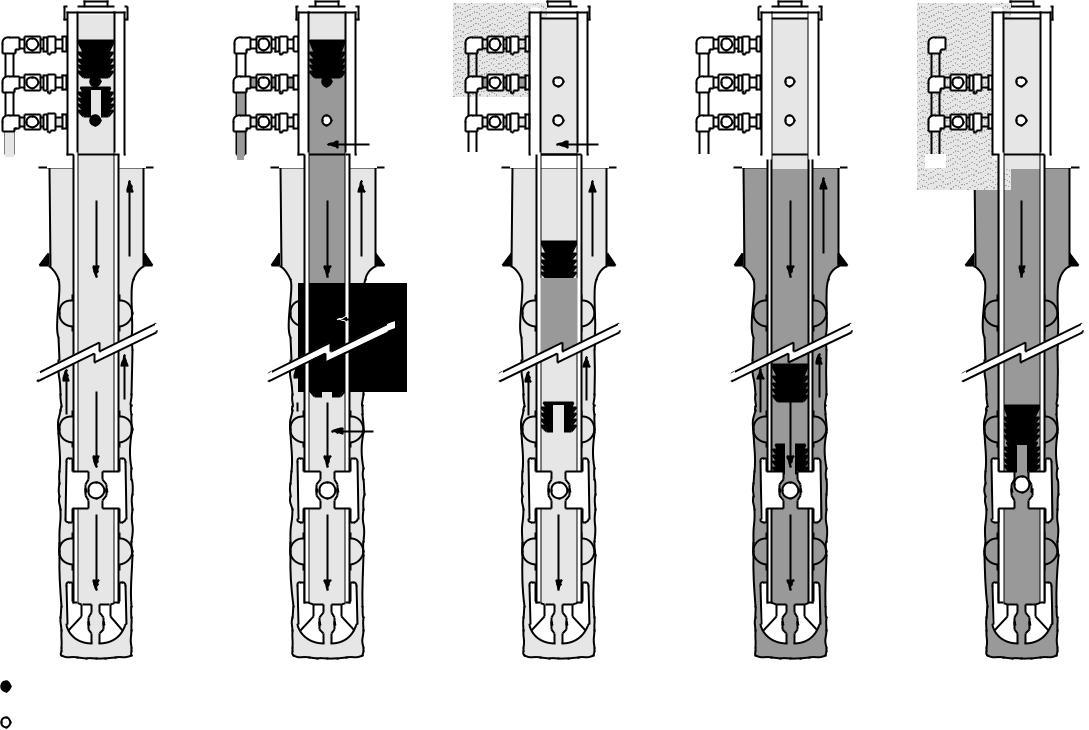
\includegraphics[scale=0.3]{images/primarycemtingoperation}
\centering 
\caption{A Picture of primary cementing operations}
\end{figure}

Cementing is performed when the cement slurry is deployed into the well via pumps,
displacing the drilling fluids still located within the well, and replacing them with cement.
The cement slurry flows to the bottom of the wellbore through the casing, 
which will eventually be the pipe through which the hydrocarbons flow to the surface. 
From there it fills in the space between the casing and the actual wellbore,
and hardens. This creates a seal so that outside materials cannot enter the well flow, as well as permanently positions the casing in place.

\vspace{1em}

\noindent \textbf{PREPARING THE CEMENT:}

\vspace{1em}

In preparing a well for cementing, it is important to establish the amount of cement required for the job.
This is done by measuring the diameter of the borehole along its depth, 
using a caliper log. Utilizing both mechanical and sonic means,
multi finger caliper logs measure the diameter of the well at numerous locations simultaneously in order to accommodate for irregularities in the wellbore diameter and determine the volume of the open hole.
Additionally, the required physical properties of the cement are essential before commencing 
cementing operations. The proper set cement is also determined, 
including the density and viscosity of the material, before actually pumping the cement into the hole.

\vspace{1em}

Special mixers, including hydraulic jet mixers, recirculating mixers or batch mixers,
are used to combine dry cement with water to create the wet cement, also known as slurry. 
The cement used in the well cementing process is Portland cement, and it is calibrated 
with additives to form one of eight different API classes of cement. Each is employed for various situations.
Additives can include accelerators, which shorten the setting time required for the cement,
as well as retarders, which do the opposite and make the cement setting time longer.
In order to decrease or increase the density of the cement, lightweight and heavyweight additives are added.

\vspace{2em}

Additives can be added to transform the compressive strength of the cement,
as well as flow properties and dehydration rates. Extenders can be used to 
expand the cement in an effort to reduce the cost of cementing, and antifoam additives
can be added to prevent foaming within the well. In order to plug lost circulation zones, 
bridging materials are added, as well.

\vspace{1em}

\noindent \textbf{CEMENTING THE WELL}

\vspace{1em}

After casing, or steel pipe, is run into the well, an L-shaped cementing 
head is fixed to the top of the wellhead to receive the slurry from the pumps. 
Two wiper plugs, or cementing plugs, that sweep the
inside of the casing and prevent mixing: the bottom plug and the top plug.
Keeping the drilling fluids from mixing with the cement slurry, 
the bottom plug is introduced into the well, and cement slurry is pumped into the well behind it. 
The bottom plug is then caught just above the bottom of the wellbore by the float collar, 
which functions as a one-way valve allowing the cement slurry to enter the well.
Then the pressure on the cement being pumped into the well is increased until a diaphragm is broken within the bottom plug,
permitting the slurry to flow through it and up the outside of the casing string.Figure 5.2 shows the images of Top  Plug and Bottom Plug

\vspace{1em}

\begin{figure}[h]
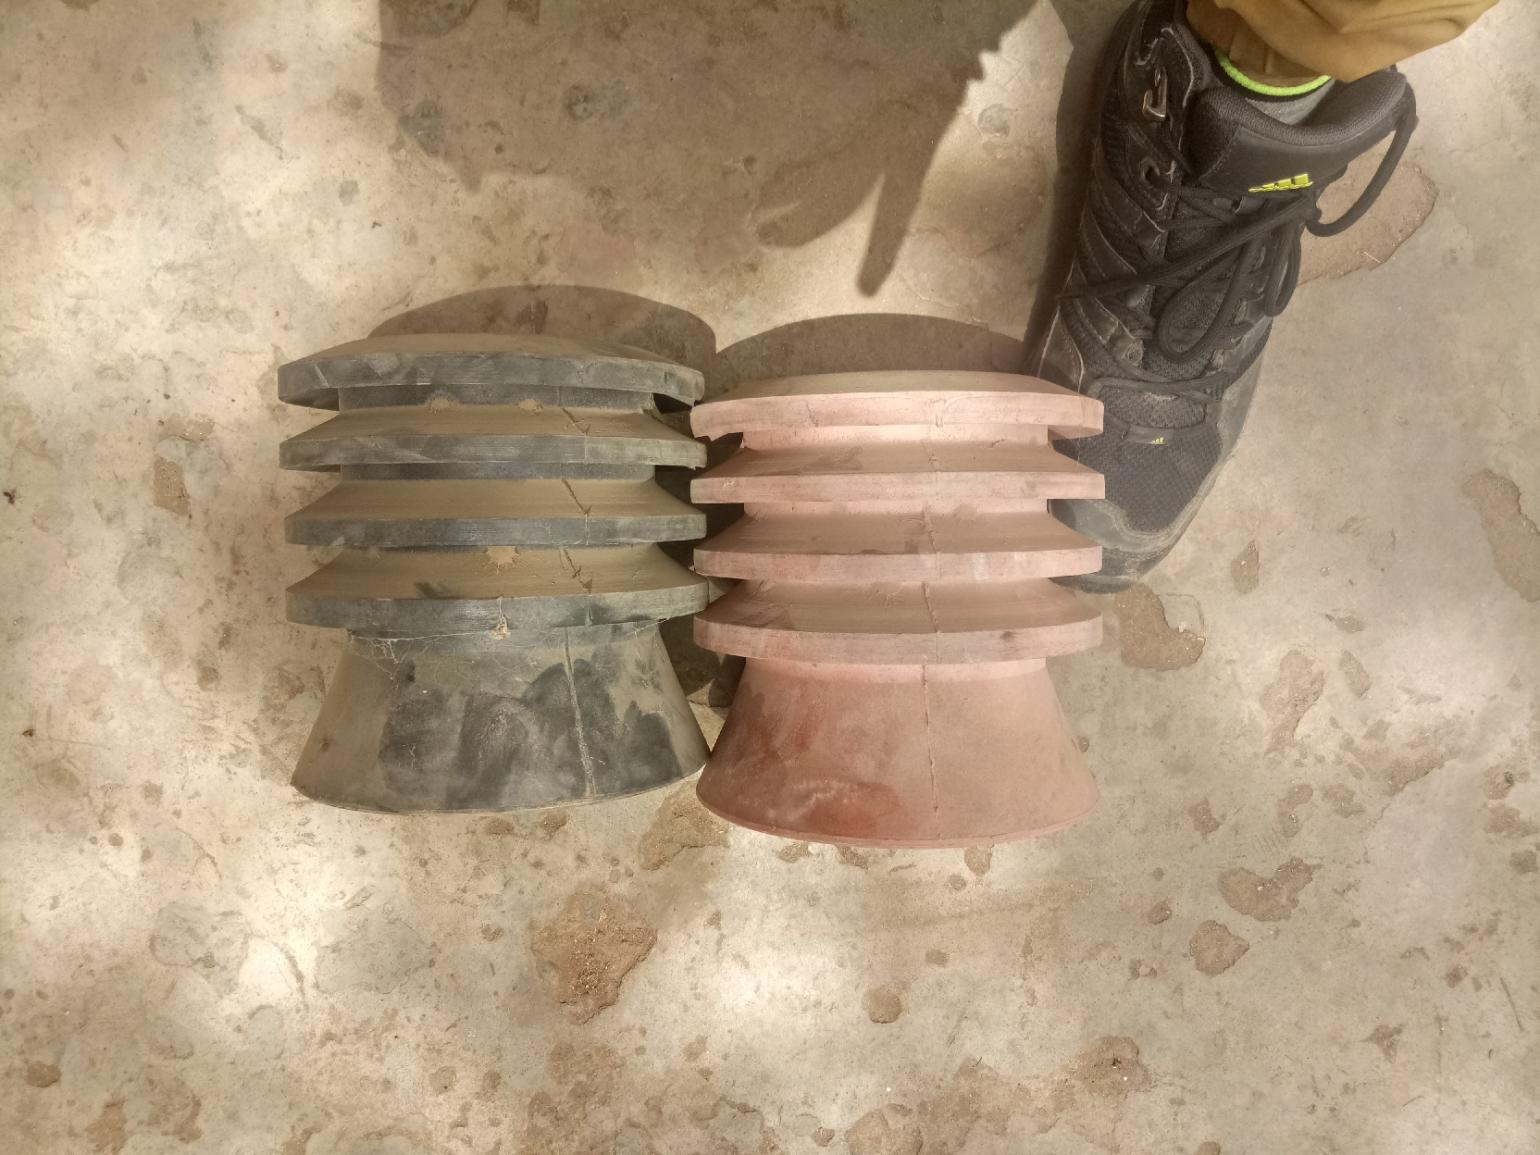
\includegraphics[scale=0.2]{images/top_plugandbottom_plug}
\centering 
\caption{A Picture of Top plug and Bottom plug}
\end{figure}

%figure of the top plug and bottom plug have to included 

After the proper volume of cement is pumped into the well, a top plug is pumped into 
the casing pushing the remaining slurry through the bottom plug.
Once the top plug reaches the bottom plug, the pumps are turned off, and the cement is allowed to set.
The amount of time it takes cement to harden is called thickening time or pump ability time. 
For setting wells at deep depths, under high temperature or pressure, as well as in corrosive environments,
special cements can be employed.


    